\documentclass{beamer}
\usetheme{Warsaw}

\title{DevOps as culture: what the history of DevOps can teach us about its implementation}
\author{Jacob Archambault}
\AtBeginSubsection[]
{
	\begin{frame}<beamer>{Outline}
		\tableofcontents[currentsection, currentsubsection]
	\end{frame}
}

\begin{document}
	\begin{frame}[plain]
		\titlepage
	\end{frame}
	\begin{frame}{Outline}
		\tableofcontents[pausesections]
		% You might wish to add the option [pausesections]
	\end{frame}
	\section{Challenges for DevOps today}
	\subsection{For developers and enquirers}
	\begin{frame}{DevOps challenges: developers and inquirers}
		\begin{itemize}\item 	Overwhelming amount of toolchain growth \pause
			\item added complexity \pause
			\item doesn't feel like I'm going faster or solving problems.\pause
			\item Meaning of DevOps is opaque \pause
			\begin{itemize}
				\item CI/CD pipeline management \pause
				\item Docker, Kubernetes, Terraform \pause
				\item Identity and access permissions \pause
				\item AWS, Azure, Google Cloud 
			\end{itemize}
		\end{itemize}
	\end{frame}
	\subsection{For business}
	\begin{frame}{DevOps challenges: business}
		\begin{itemize}
			\item DevOps engineers are among the highest paid positions outside of management
			\pause
			\item Not using DevOps technologies poses a flight risk \pause
		\end{itemize}
	\end{frame}
	\subsection{Common challenges}
	\begin{frame}{DevOps challenges: avoiding a worst-of-all-worlds scenario}
		\begin{itemize}
			\item increased operating costs from hiring more experienced developers \pause
			\item added unnecessary complexity in our dev stack \pause
			\item restricted the freedom of developers to actually get stuff done \pause
			\item forfeited ownership of our infrastructure \pause 
			\item rebranded our operations team
		\end{itemize}
	\end{frame}
	\section{A short history of DevOps}
	\subsection{its beginning}
	\begin{frame}{DevOps: its beginning}
		\begin{itemize}
			\item Velocity Conference 2009: John Allspaw and Paul Hammond, "10+ Deploys Per Day: Dev and Ops Cooperation at Flickr" \pause
			\item Patrick Debois \href{https://youtu.be/EOveXZhJpr4}{DevOps Days 2009, Ghent, Belgium}
		\end{itemize}
	\end{frame}
	\subsection{its roots}
	\subsubsection{Throughput}
	\begin{frame}{Goldratt's theory of constraints}
		\begin{itemize}
			\item Increase: throughput \pause
			\item Decrease: \pause
			\begin{itemize}
				\item operating costs \pause
				\item inventory \pause
				\item scrap \pause
			\end{itemize}
			\item Remove bottlenecks
		\end{itemize}
	\end{frame}
	\begin{frame}{Goldratt's theory of constraints (cont.)}
		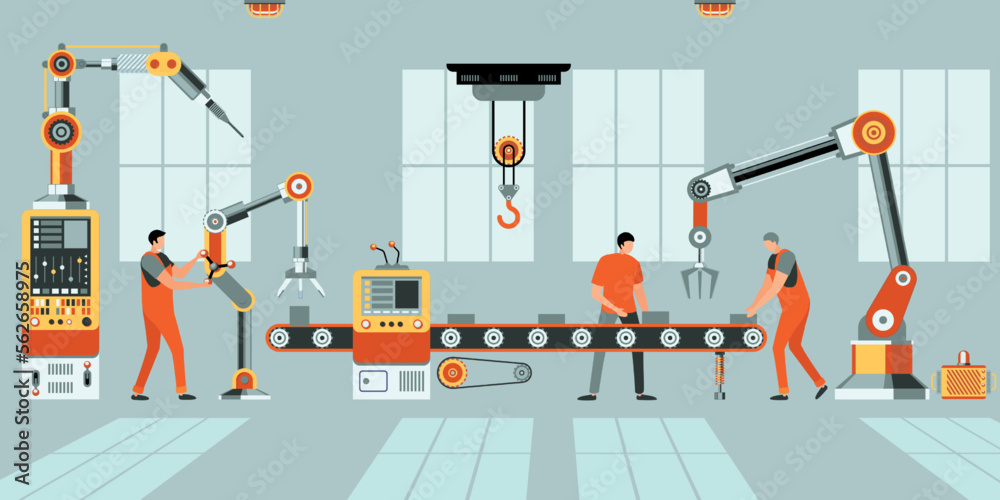
\includegraphics{assemblyline}
	\end{frame}
	\subsubsection{Communication}
	\begin{frame}{1967: Conway's law}
		\begin{quote}
			`Organizations which design systems [...] are constrained to produce designs which are copies of the communication structures of these organizations.' - Melvin Conway, `How do Committees Invent?' Datamation, 1967
		\end{quote}
	\end{frame}
	\begin{frame}{Conway's law: examples}
		\begin{itemize}
			\item `If you have four groups working on a compiler, you'll get a 4-pass compiler' - The New Hacker's Dictionary, 1996\pause
			\item front-end [devs] business layer [backend devs] monolithic database [DBA team] \pause
			\item a web api controller [manager]  delegates most business logic to business classes [developers] which are part of the same in-memory process [team], while serving as a single entry-point for wider cross-network [cross-team] communication.
		\end{itemize}
	\end{frame}
	\begin{frame}{1975: The Mythical Man Month, Fred Brooks}
		
		\begin{itemize}
			\item number of direct communication paths for $n$ individuals= $n(n-1)/2$
		\end{itemize}
		\begin{center}
			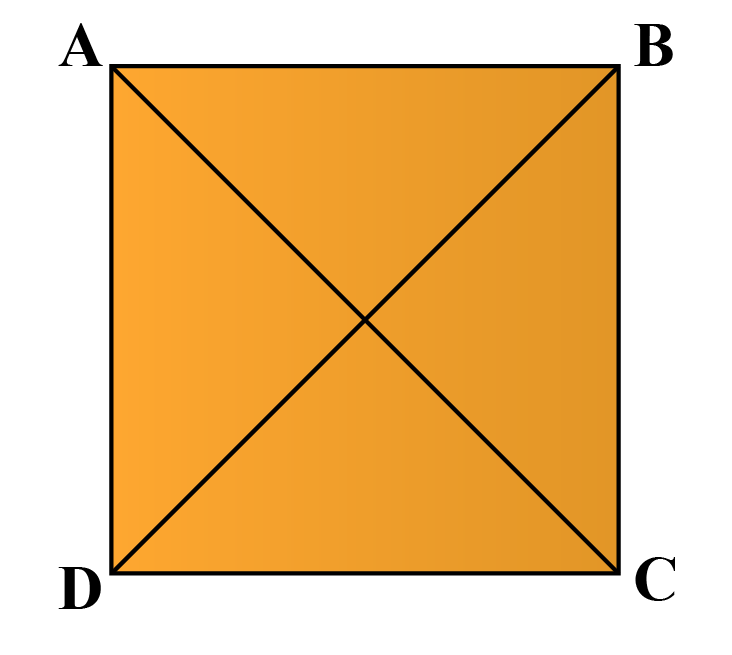
\includegraphics[width=.5\textwidth]{square}
		\end{center}
		
	\end{frame}
	\begin{frame}{1975: The Mythical Man Month, Fred Brooks}
		
		\begin{itemize}
			\item number of direct communication paths for $n$ individuals= $n(n-1)/2$
		\end{itemize}
		\begin{center}
			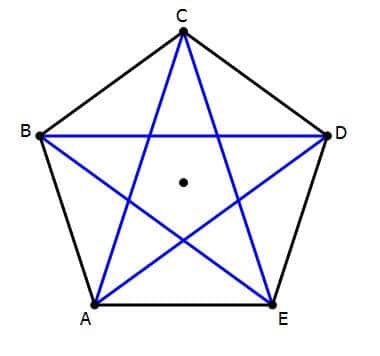
\includegraphics[width=.5\textwidth]{pentagon}
		\end{center}
		
	\end{frame}
	\begin{frame}{1975: The Mythical Man Month, Fred Brooks}
		
		\begin{itemize}
			\item number of direct communication paths for $n$ individuals= $n(n-1)/2$
		\end{itemize}
		\begin{center}
			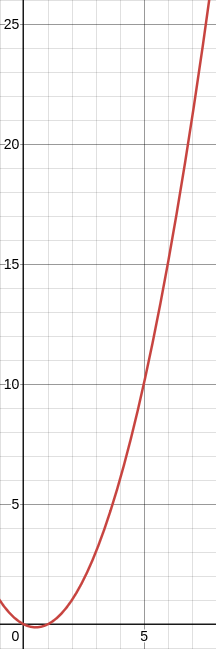
\includegraphics[width=.15\textwidth]{graph}
		\end{center}
	\end{frame}
	\begin{frame}{The Mythical Man Month, Fred Brooks (cont.)}
			\begin{itemize}
				\item corollary: adding more people to a project can lead not only to diminishing returns on delivery speed, but to objectively less work being completed
			\end{itemize}
		\end{frame}
	\end{document}
